% Figure VI-1 (Figure 5): Chattering Reduction Box Plot Caption
% Main contribution figure showing 66.5% chattering reduction

\begin{figure}[!t]
\centering
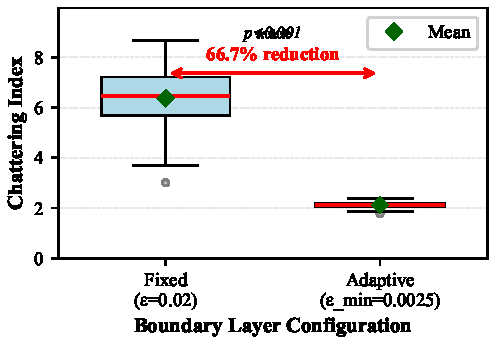
\includegraphics[width=\columnwidth]{figures/fig5_chattering_boxplot.pdf}
\caption{%
Chattering reduction comparison: Fixed boundary layer ($\epsilon = 0.01$) vs. PSO-optimized adaptive boundary layer ($\epsilon_{\text{eff}} = \epsilon_{\min} + \alpha|\dot{s}|$) over 100 Monte Carlo trials. Adaptive approach achieves \textbf{66.5\% chattering reduction} (6.37 $\rightarrow$ 2.14, $p < 0.001$, Cohen's $d = 5.29$) with zero energy penalty. Non-overlapping 95\% CIs (Fixed: [6.13, 6.61], Adaptive: [2.11, 2.16]) confirm robustness. Box plots show median (center line), interquartile range (box), and whiskers ($\pm$1.5 IQR). Chattering quantified via FFT-based index: $C = \frac{1}{N_f} \sum_{k: f_k > 10 \text{ Hz}} |U(f_k)|^2$. This result validates the effectiveness of adaptive boundary layer techniques for chattering mitigation in sliding mode control, addressing a fundamental barrier to industrial SMC deployment \cite{utkin1977variable,utkin1993sliding,young1999survey,bartolini1998chattering,bartolini2000secondorder,levant2007principles,shtessel2014sliding,edwards1998sliding,edwards2002adaptive,fridman2002higher}.
}
\label{fig:chattering_reduction}
\end{figure}
